\chapter{EVALUATION}
\label{sect:evaluation}
We conduct experiments on \pf using probability computation algorithm mentioned in Algorithm \ref{alg:prob} and compare results with \TPR.
\section{Experimental setup info}
The objects data are provided from real Washington state moving objects data. The section is divided into accuracy experiments, efficiency experiments and finally scalability experiments. The experiments were run on an Intel Core i7 2.4GHz CPU with 12GB RAM under Windows 8.1.
\section{Accuracy Evaluation}
\begin{itemize}
\item what is the chart about
\item what is x and y axises represent
\item describe our assumptions and constants: number of nodes, number of quires, etc..
\item describe \pf algorithm trend
\item describe \tpr algorithm trend
\item compare \pf and \tpr algorithms results
\item conclusion from the comparison (why \pf outstand \tpr)
\item describe/imagine any peak/strange values
\item describe how the chart will be changed when adjusting parameters.
\end{itemize}

%The accuracy experiments evaluate how much the prediction algorithm is accurate given the uncertainty. The input parameter to the experiments is the region radius in kilometer and the number of prediction steps. The results radius 0, 0.05, and 0.1 radius variations are shown in Figure ~\ref{fig:accuracy}. In Figure ~\ref{fig:accuracy0} the probability of the prediction for \pf is getting more accurate by time while \tpr prediction remains constant over time. This is resulted from the pruning operation that's applied for the \pf while reduces the search space for the algorithm to get more accurate results.
%By looking into the overall results in Figure ~\ref{fig:accuracy} it's notable how \pf sustains good prediction probability when the uncertainty is increased by increasing the region size. This is gained by having the assumption that user moves in a shortest path which enables the update algorithm to neglect paths that are not promising or won't result in a shortest path.

\begin{figure*}[ht]
\centering
\subfigure[Region radius 0 kilometer.]{
\vtop{\vskip0pt
\hbox{
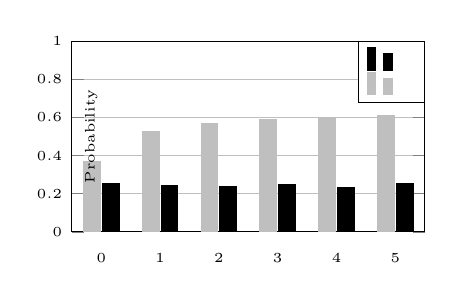
\begin{tikzpicture}
    \begin{axis}[
        width  = 0.5 * \textwidth,
        height = 4cm,
        major x tick style = transparent,
        ybar= 2 * \pgflinewidth,
        bar width=6pt,
        ymajorgrids = true,
        ylabel = {Probability},
        y label style={font=\tiny, at={(0.1,0.5)}},
        symbolic x coords={0, 1, 2, 3, 4, 5},
        x tick label style= {
                font=\tiny
            },
            y tick label style= {
                font=\tiny
            },
        xtick = data,
        scaled y ticks = false,
        enlarge x limits=0.1,
        ymin=0,
        ymax=1,
        legend cell align=left,
        every node near coord/.append style={font=\tiny},
        legend style={
                at={(1.0,1.0)},
                anchor=north east,
                column sep=1ex
        },
        reverse legend
    ]
        \addplot[style={lightgray,fill=lightgray,mark=none}]
            coordinates {
                (0, 0.3662)
                (1, 0.5267) % 0.6267
                (2, 0.5671) % 0.06471
                (3, 0.5889) % 0.6489
                (4, 0.6009) % 0.6489
                (5, 0.6100) % 0.6448
        };

        \addplot[style={black,fill=black,mark=none}]
             coordinates {
                (0, 0.2529)
                (1, 0.2412)
                (2, 0.2389)
                (3, 0.2494)
                (4, 0.2326)
                (5, 0.2545)
         };

        \legend{\tiny \PF, \tiny \TPR}
    \end{axis}
\end{tikzpicture}
\label{fig:accuracy0}
}
}}
\subfigure[Region radius 0.05 kilometer.]{
\vtop{\vskip0pt
\hbox{
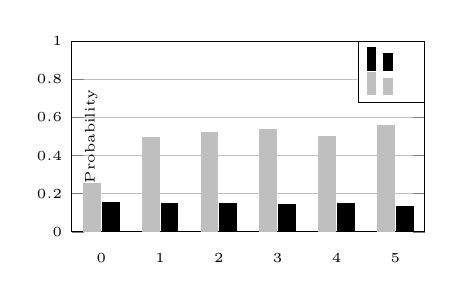
\begin{tikzpicture}
    \begin{axis}[
        width  = 0.5 * \textwidth,
        height = 4cm,
        major x tick style = transparent,
        ybar= 2 * \pgflinewidth,
        bar width=6pt,
        ymajorgrids = true,
        ylabel = {Probability},
        y label style={font=\tiny, at={(0.1,0.5)}},
        symbolic x coords={0, 1, 2, 3, 4, 5},
        x tick label style= {
                font=\tiny
            },
            y tick label style= {
                font=\tiny
            },
        xtick = data,
        scaled y ticks = false,
        enlarge x limits=0.1,
        ymin=0,
        ymax=1,
        legend cell align=left,
        every node near coord/.append style={font=\tiny},
        legend style={
                at={(1.0,1.0)},
                anchor=north east,
                column sep=1ex
        },
        reverse legend
    ]
        \addplot[style={lightgray,fill=lightgray,mark=none}]
            coordinates {
                (0, 0.2510)
                (1, 0.4924)
                (2, 0.5208)
                (3, 0.5383)
                (4, 0.4977)
                (5, 0.5568)
        };

        \addplot[style={black,fill=black,mark=none}]
             coordinates {
                (0, 0.1516)
                (1, 0.1501)
                (2, 0.1468)
                (3, 0.1448)
                (4, 0.1459)
                (5, 0.1335)
         };

        \legend{\tiny \PF, \tiny \TPR}
    \end{axis}
\end{tikzpicture}
\label{fig:accuracy05}}
}}
\subfigure[Region radius 0.1 kilometer.]{
\vtop{\vskip0pt
\hbox{
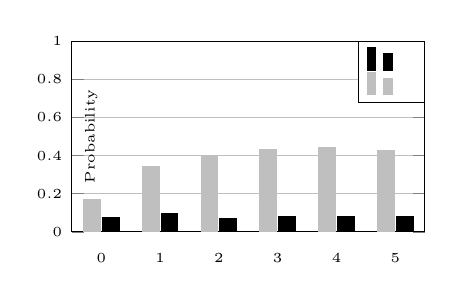
\begin{tikzpicture}
    \begin{axis}[
        width  = 0.5 * \textwidth,
        height = 4cm,
        major x tick style = transparent,
        ybar= 2 * \pgflinewidth,
        bar width=6pt,
        ymajorgrids = true,
        ylabel = {Probability},
        y label style={font=\tiny, at={(0.1,0.5)}},
        symbolic x coords={0, 1, 2, 3, 4, 5},
        x tick label style= {
                font=\tiny
            },
            y tick label style= {
                font=\tiny
            },
        xtick = data,
        scaled y ticks = false,
        enlarge x limits=0.1,
        ymin=0,
        ymax=1,
        legend cell align=left,
        every node near coord/.append style={font=\tiny},
        legend style={
                at={(1.0,1.0)},
                anchor=north east,
                column sep=1ex
        },
        reverse legend
    ]
        \addplot[style={lightgray,fill=lightgray,mark=none}]
            coordinates {
                (0, 0.1717)
                (1, 0.3444)
                (2, 0.4007)
                (3, 0.4339)
                (4, 0.4446)
                (5, 0.4275)
        };

        \addplot[style={black,fill=black,mark=none}]
             coordinates {
                (0, 0.0740)
                (1, 0.0951)
                (2, 0.0681)
                (3, 0.0806)
                (4, 0.0819)
                (5, 0.0801)
         };

        \legend{\tiny \PF, \tiny \TPR}
    \end{axis}
\end{tikzpicture}
\label{fig:accuracy1}
}
}}
\caption{Accuracy experiments for different region sizes}
\label{fig:accuracy}
\end{figure*}

\section{Scalability and Efficiency Evaluation}
The scalability experiments are applied to reveal how much \pf is scalable with respect of changing input parameters like radius size. In every experiment we scale one parameter and keep the others constants unchanged. The plots for the scalability experiments for CPU usage are in Figure ~\ref{fig:scalaCpu} and memory usage in Figure ~\ref{fig:scalaMem}

\begin{figure*}[ht]
\centering
\subfigure[Region Size.]{
\vtop{\vskip0pt
\hbox{
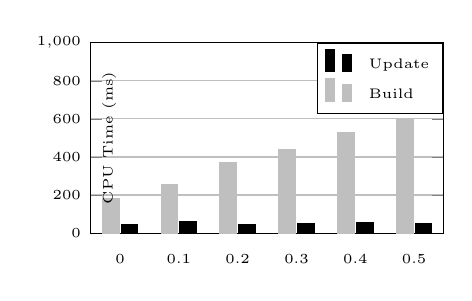
\begin{tikzpicture}
    \begin{axis}[
        width  = 0.5 * \textwidth,
        height = 4cm,
        major x tick style = transparent,
        ybar= 2 * \pgflinewidth,
        bar width=6pt,
        ymajorgrids = true,
        ylabel = {CPU Time (ms)},
        y label style={font=\tiny, at={(0.1,0.5)}},
        symbolic x coords={0, 0.1, 0.2, 0.3, 0.4, 0.5},
        x tick label style= {
                font=\tiny
            },
            y tick label style= {
                font=\tiny
            },
        xtick = data,
        scaled y ticks = false,
        enlarge x limits=0.1,
        ymin=0,
        ymax=1000,
        legend cell align=left,
        every node near coord/.append style={font=\tiny},
        legend style={
                at={(1.0,1.0)},
                anchor=north east,
                column sep=1ex
        },
        reverse legend
    ]
        \addplot[style={lightgray,fill=lightgray,mark=none}]
            coordinates {
                (0, 183.1303)
                (0.1, 253.7468) %753
                (0.2, 368.9956) % 1368
                (0.3, 436.7922) % 3236
                (0.4, 526.7508) % 4926
                (0.5, 602.3495) % 7402

        };
        \addplot[style={black,fill=black,mark=none}]
             coordinates {
                (0, 47.0653)
                (0.1, 63.0394)
                (0.2, 47.0371)
                (0.3, 52.1937)
                (0.4, 55.5097)
                (0.5, 52.0552)
         };

        \legend{\tiny Build, \tiny Update}
    \end{axis}
\end{tikzpicture}
\label{fig:scalaCpu0}
}}}
\caption{Scalability CPU Usage Experiments for \PF}
\label{fig:scalaCpu}
\end{figure*}

\begin{figure*}[ht]
\centering
\subfigure[Region Size.]{
\vtop{\vskip0pt
\hbox{
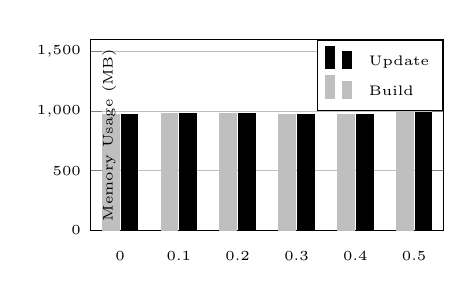
\begin{tikzpicture}
    \begin{axis}[
        width  = 0.5 * \textwidth,
        height = 4cm,
        major x tick style = transparent,
        ybar= 2 * \pgflinewidth,
        bar width=6pt,
        ymajorgrids = true,
        ylabel = {Memory Usage (MB)},
        y label style={font=\tiny, at={(0.1,0.5)}},
        symbolic x coords={0, 0.1, 0.2, 0.3, 0.4, 0.5},
        x tick label style= {
                font=\tiny
            },
            y tick label style= {
                font=\tiny
            },
        xtick = data,
        scaled y ticks = false,
        enlarge x limits=0.1,
        ymin=0,
        ymax=1600,
        legend cell align=left,
        every node near coord/.append style={font=\tiny},
        legend style={
                at={(1.0,1.0)},
                anchor=north east,
                column sep=1ex
        },
        reverse legend
    ]
        \addplot[style={lightgray,fill=lightgray,mark=none}]
            coordinates {
                (0, 973.8984375)
                (0.1, 976.46875)
                (0.2, 979.4140625)
                (0.3, 975.7109375)
                (0.4, 972.296875)
                (0.5, 991.19140625)

        };
        \addplot[style={black,fill=black,mark=none}]
             coordinates {
                (0, 973.8984375)
                (0.1, 976.46875)
                (0.2, 979.4140625)
                (0.3, 975.7109375)
                (0.4, 972.296875)
                (0.5, 991.19140625)
         };

        \legend{\tiny Build, \tiny Update}
    \end{axis}
\end{tikzpicture}
\label{fig:scalaMem0}
}}}
\caption{Scalability Memory Usage Experiments for \PF}
\label{fig:scalaMem}
\end{figure*}